Для наблюдения дифракции Фраунгофера на двух щелях в установке
рис. \ref{img:scheme1} следует заменить щель $S_2$ экраном $Э$ с двумя щелями рис. \ref{img:slits}.
При этом для оценки влияния ширины входной щели на чёткость дифракционной картины вместо входной щели $S_1$следует поставить щель
с микрометрическим винтом. Два дифракционных изображения входной
щели, одно из которых образовано лучами, прошедшими через левую, а
другое ~---~ через правую щели, накладываются друг на друга.
Если входная щель достаточно узка, то дифракционная картина
в плоскости $\Pi$ рис. \ref{img:slits} подобна той, что получалась при дифракции на
одной щели рис. \ref{img:scheme1}, однако теперь вся картина испещрена рядом дополнительных узких полос. Наличие этих полос объясняется суперпозицией
световых волн, приходящих в плоскость наблюдения через разные щели

\begin{figure}[h]
  \center{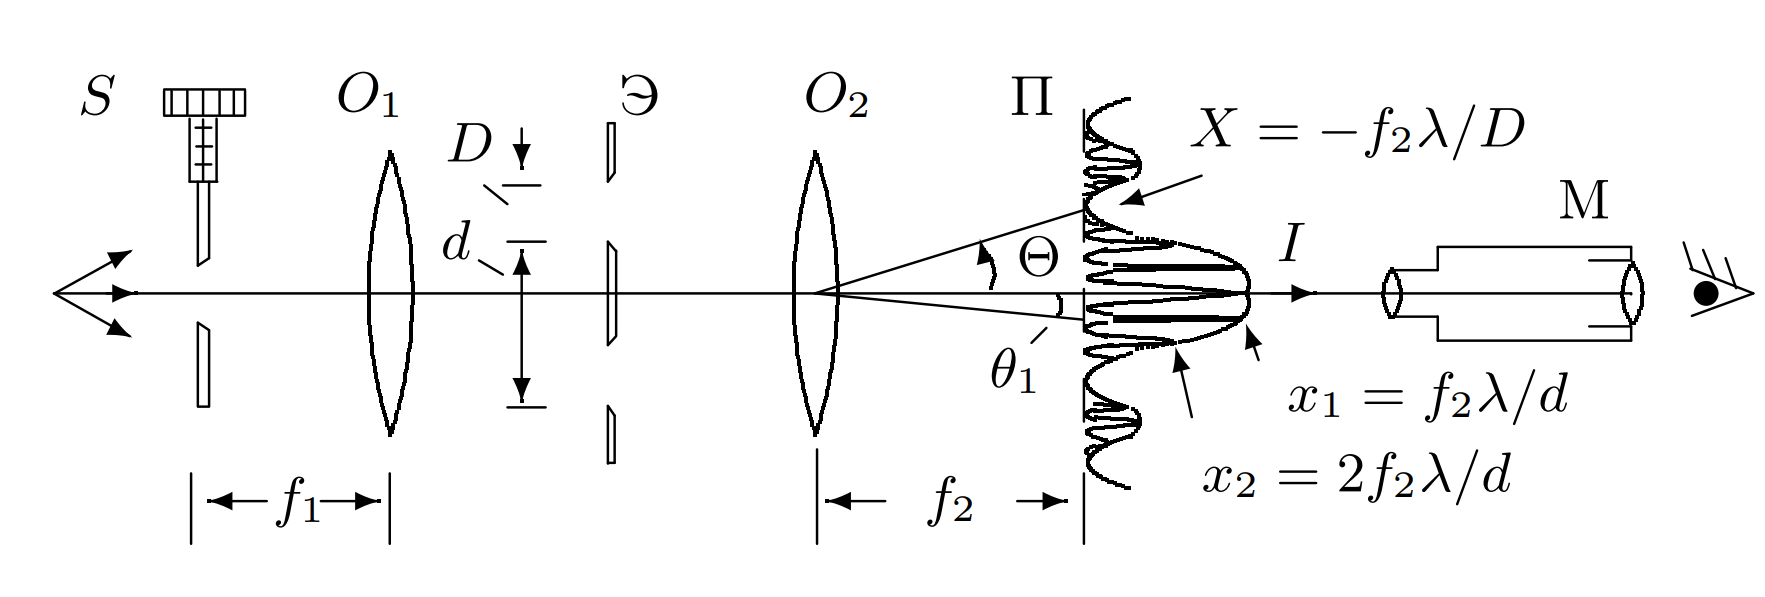
\includegraphics[width=1\linewidth]{two_slit.png}}
  \caption{Схема установки для наблюдения дифракции Фраунгофера на двух щелях}
  \label{img:slits}
\end{figure} 
\
экрана Э. В центре главного дифракционного максимума рис. \ref{img:slits} располагается светлая полоса, так как при $\theta = 0$ разность хода между этими
волнами равна нулю (все лучи, приходящие в фокус объектива $O_2$ , синфазны). Светлая интерференционная полоса наблюдается и во всех тех
случаях, когда указанная разность хода равна целому числу длин волн.
Таким образом, угловая координата $\theta_m$ интерференционного максимума $m$-го порядка определяется соотношением

\begin{equation}
  d \cdot \theta_m = m\lambda,
\end{equation} \label{eq:fraunmax}
\
где $d$ ~---~ расстояние между щелями.
Линейное расстояние $\delta x$ между соседними интерференционными 
полосами в плоскости $\Pi$ равно поэтому

\begin{equation}
  \delta x = f_2 \frac{\lambda}{d}.
\end{equation} \label{eq:fraundx}

На рис. \ref{img:slits} показано распределение интенсивности в фокальной 
плоскости объектива $O_2$. Штриховой линией (в увеличенном масштабе) 
изображено распределение интенсивности при дифракции света на одиночной
щели.
Нетрудно оценить число $n$ интерференционных полос, 
укладывающихся в области центрального дифракционного максимума. 
Согласно \eqref{eq:dist_m} полная ширина главного максимума равна $ 2f_2 \lambda /D$, где $D$ ~---~ 
ширина щели, отсюда
\begin{equation}
  n = \frac{2\lambda f_2}{D} \frac{1}{\delta x} = \frac{2d}{D}.
\end{equation}\label{eq:intnum}

При дифракции света на двух щелях чёткая система 
интерференционных полос наблюдается только при достаточно узкой ширине входной
щели $S$. При увеличении её ширины интерференционная картина 
периодически пропадает и появляется вновь, но полосы при этом оказываются
сильно размытыми и видны плохо. Это явление объясняется 
наложением интерференционных картин от разных элементов широкой щели $S$.
Первое размытие интерференционных полос возникает при условии
\begin{equation}
  \frac{b}{f_1} =\frac{\lambda}{d}.
\end{equation}\label{eq:intblur}

Здесь $b$ — ширина входной щели
$S$ и, следовательно, $b/f_1$ ~---~ её угловая ширина.
Таким образом, по размытию интерференционной
картины
можно оценить размер источника. Этот метод используется в звёздном
интерферометре при измерении угловых размеров звёзд.